 

 %in preamble
 %%%%% DIRECTION FIELDS %%%%%%%%%
\pgfplotsset{ % Define a common style, so we don't repeat ourselves
    MaoYiyi/.style={
        width=0.6\textwidth, % Overall width of the plot
        axis equal image, % Unit vectors for both axes have the same length
        view={0}{90}, % We need to use "3D" plots, but we set the view so we look at them from straight up
        xmin=-4, xmax=4, % Axis limits
        ymin=-4, ymax=4,
        domain=-4:4, y domain=-4:4, % Domain over which to evaluate the functions
        xtick={-4,0,4}, ytick={-4,0,4}, % Tick marks
        samples=22, % How many arrows?
        cycle list={    % Plot styles
                gray,
                quiver={
                    u={1}, v={f(x,y)}, % End points of the arrows
                    scale arrows=0.095,
                    every arrow/.append style={
                        -latex % Arrow tip
                    },
                }\\
                red, samples=31, smooth, thick, no markers, domain=-4:4\\ % The plot style for the function
        }
    }
}
%%%%% DIRECTION FIELDS %%%%%%%%%

 
 
 
 
 %in document
 
 
\begin{tikzpicture}[
    declare function={f(\x,\y) = 0.2*\x*\y;} % Define which function we're using
]
\begin{axis}[
    MaoYiyi, title={$\dfrac{\mathrm{d}y}{\mathrm{d}x} = 0.2 x y $}
]
\addplot3 (x,y,0);
\addplot {e^(0.1*x^2)}; % You need to find the antiderivative yourself, unfortunately. Good exercise!
\end{axis}
\end{tikzpicture}
